\documentclass{article}
\usepackage{graphicx}
\usepackage{amsmath}
\usepackage{float}
\usepackage{amssymb} % Simbolos matematicos (por lo tanto)
\usepackage{longtable} %agregadom para hacer tablas
\usepackage{xltabular}
\usepackage{tabularray}
\usepackage{graphicx} % Incluir imágenes en LaTeX
\graphicspath{ {./images/} }

\begin{document}

\newpage
\section*{1. Introducción y objetivos del experimento}
Este informe se basa en datos obtenidos en el laboratorio de Física II de la Facultad de Ciencias. Se fundamenta en la guía de laboratorio y otras referencias citadas más adelante. Su objetivo es responder el cuestionario y comparar los resultados experimentales con la teoría. De acuerdo con la guía del laboratorio y las instrucciones del docente, el informe se organiza como sigue.


\section*{2. Fundamento teórico}
\subsection*{2.1. Energía cinética de rotación y traslación}
La energía cinética se expresa como:
\begin{equation*}
E_{c} = \frac{1}{2} m v^{2}
\end{equation*}

\begin{figure}[H]
    \centering
        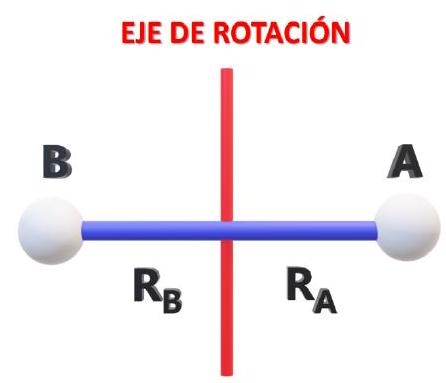
\includegraphics[scale=0.30]{2025_04_01_ea720b93e8ebb5d0c6aeg-03}
    \caption{Ejemplo de imagen}
\end{figure}

Consideremos un sistema de dos cuerpos A y B unidos por una barra de masa insignificante que giran alrededor de un eje perpendicular a la barra con velocidad angular $\vec{w}$. La energía cinética del sistema es:

\begin{equation*}
E_{c} = \frac{1}{2} m_{A} w^{2} R_{A}^{2} + \frac{1}{2} m_{B} w^{2} R_{B}^{2}
\end{equation*}

\subsection*{2.2. Momento de inercia}
Factorizando $\frac{1}{2} w^{2}$, tenemos:

\begin{equation*}
E_{c} = \frac{1}{2} I w^{2}
\end{equation*}

donde el momento de inercia del sistema respecto al eje es:

\begin{equation*}
I = \sum_{i=1}^{n} m_{i} R_{i}^{2}
\end{equation*}

Para un sistema continuo:

\begin{equation*}
I = \int r^{2} dm
\end{equation*}

\begin{figure}[H]
    \centering
    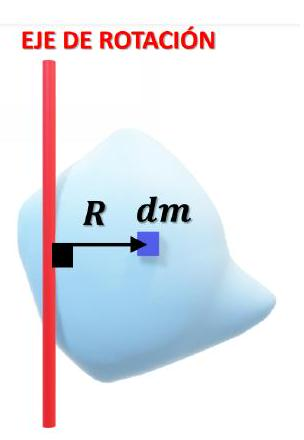
\includegraphics[scale=0.30]{2025_04_01_ea720b93e8ebb5d0c6aeg-05}
    \caption{Sistema de masas continuo}
\end{figure}

\begin{figure}[H]
    \centering
    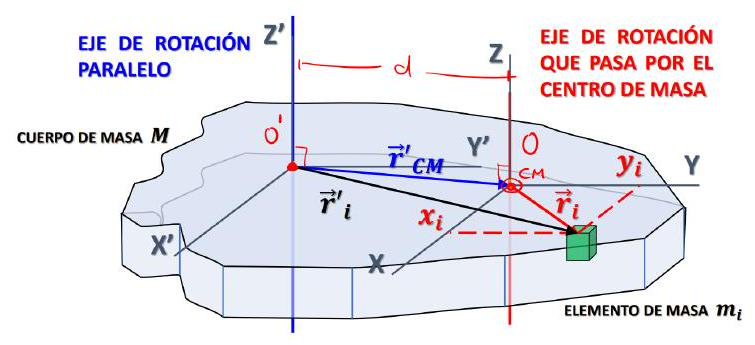
\includegraphics[scale=0.30]{2025_04_01_ea720b93e8ebb5d0c6aeg-05(1)}
    \caption{Lámina plana del objeto}
\end{figure}

Donde $\overrightarrow{r_{i}}$ representa la posición del elemento de masa $m_{i}$ respecto al centro de masa, mientras que $\overrightarrow{r_{i}}^{\prime}$ es la posición respecto a un eje paralelo. 

\end{document}
